% !TEX spellcheck = en_US

% !TEX root = elastophi-report.tex


\section{Low rank approximations}
\label{sec:LowRankApprox}

In this section we are interested in fully populated matrices $\mA\in \C^{n\times n}$, $\mA = (\mA_{j,k})_{j,k=1\dots n}$ with, a priori, 
none of its entries vanishing, its size $n$ being potentially large. With no particular assumption on this matrix, the cost of a 
matrix-vector product is $\mathcal{O}(n^{2})$. 

\bigskip
This cost is substantially reduced if we assume that $\mA$ is of low rank though. We say that a matrix has the low rank property, 
with rank $k\leq n$, if there exist vectors $\bfu_{j},\bfv_{j}\in \C^{n}, j=1\dots k$, such that 
\[
\mA = \sum_{j=1}^{k}\bfu_{j}\cdot\bfv_{j}^{T}\quad \textrm{with}\quad k\leq n/2.
\]
Indeed if this representation holds, then a matrix-vector product requires $2 k n$ flops, which is smaller than $n^{2}$ provided 
that the condition on $k$ given above is satisfied. Matrices $\mA$ encountered in applications rarely have the low rank property. 
A simple primary observation is that general matrices $\mA$ can be written as a sum of rank one matrices through its singular value
decomposition
\begin{equation}\label{SVD}
\mA = \sum_{j=1}^{n}\sigma_{j}\,\bfu_{j}\cdot\bfv_{j}^{T}\quad \textrm{where}\;\; \mathfrak{S}(\mA^{*}\mA) = \{\sigma_{j}^{2}\}_{j=1\dots n},
\end{equation}
where $(\bfu_{j})_{j=1}^{n}, (\bfv_{j})_{j=1}^{n}$ are orthonormal basis of $\C^{n}$ and $\sigma_{1}\geq \sigma_{2}\geq \dots \geq \sigma_{n}$. 
A closer inspection of this formula leads to the conclusion, provided that the sequence $(\sigma_{j})$  decreases fast, that 
truncating the singular value decomposition (\ref{SVD}) yields a good approximation of the matrix $\mA$. This is the essence of 
the next result.

\begin{proposition}\quad\\
Let $\mA\in \C^{n\times n}$ admit the singular value decomposition (\ref{SVD}), and denote $\mA_{k}$ the 
matrix obtained by truncating this decomposition at rank $k$ namely $\mA_{k}:=\sum_{j=1}^{k}\sigma_{j}\,\bfu_{j}
\cdot\bfv_{j}^{T}$. Then we have the error estimates
\[
\Vert \mA - \mA_{k}\Vert_{2}^{2} = \sigma_{k+1}^{2}
\quad\textrm{and}\quad 
\Vert \mA - \mA_{k}\Vert_{\mrm{F}}^{2} = \sum_{j=k+1}^{n}\sigma_{j}^{2},
\]
where $\Vert \;\Vert_{2}$ refers to the matrix norm induced by the vector norm $\vert \bfu\vert_{2} = (\sum_{j=1}^{n}\vert u_{j}\vert^{2})$ 
for $\bfu = (u_{j})_{j=1}^{n}\in \C$ and $\Vert \;\Vert_{\mrm{F}}$ refers to the Frobenius norm.
\end{proposition}

Truncating the SVD is thus an efficient way to approximate a matrix, and thus to reduce the cost of the 
matrix-vector product, provided that  the singular values decrease fast. Assume that singular values decrease 
exponentially, say $\sigma_{k}\leq q^{k}$ for a fixed $q\in (0,1)$. Then for a relative error expressed in Frobenius norm of order $\varepsilon>0$,  
it suffices to take $k \simeq \log_q \varepsilon$. 

\bigskip
Unfortunately, computing the singular value decomposition  of a matrix is expensive: it costs $\mathcal{O}(n^{3})$ flops. To circumvent this issue, starting from 
an arbitrary matrix $\mA$ whose singular values are assumed to decrease exponentially, the Adaptative 
Cross Approximation (ACA) algorithm provides a collection of vectors $\bfu_{j},\bfv_{j}\in \C^{n}, j=1\dots n$ such that 
the matrices 
\begin{align}
\label{eq:low_rank_decomposition}
\widetilde{\mA}_{k} = \sum_{j=1}^{k}\bfu_{j}\cdot\bfv_{j}^{T}
\end{align} 
satisfy 
\begin{align*}
\Vert \mA - \widetilde{\mA}_{k}\Vert_{\mrm{F}}\leq C \Vert \mA - \mA_{k}\Vert_{\mrm{F}}
\end{align*}
for some constant $C>0$ independent of $k$. Moreover, which is probably the most interesting feature of this method, 
the cost of computing $\widetilde{\mA}_{k}$ is $\mathcal{O}(kn)$. This cost is thus quasi-linear provided that the singular 
values  decrease exponentially. Besides, the algorithm does not require to generate all the coefficients of the matrix, so that the cost of the storage is also in $\mathcal{O}(kn)$. The detailed analysis of the ACA algorithm is out of the scope of this report. We only 
give the algorithm itself.

\begin{algorithm}
  \caption{Partially Pivoted ACA}  
  \label{AlgoACA}
  Initialize $j_{*}$\\
  $r=0$\\
  \textbf{while}(stopping criterion not satisfied)\{\\\quad\\
  \indent\hspace{0.5cm} \parbox{\linewidth}{
    $\bfw = \mA(j_{*},:)^{T} - \sum_{\ell=1}^{r}\bfu_{\ell}(j_{*})\,\bfv_{\ell}$\\
    $k_{*} = \mathop{\mrm{argmax}}_{k = 1\dots n}\vert \bfw(k)\vert$\\
    $w_{*} = \bfw(k_{*})$\\\quad\\
    \textbf{if}($w_{*}\neq 0$)\{\\\quad\\
    \indent\hspace{0.5cm} \parbox{\linewidth}{
      $\bfv_{r+1} = \bfw$\\
      $\bfw = \mA(:,k_{*})-\sum_{\ell = 1}^{r}\bfv_{\ell}(k_{*})\,\bfu_{\ell} $\\
      $\bfu_{r+1} = w_{*}^{-1}\bfw$\\      
      $j_{*} = \mathop{\mrm{argmax}}_{j = 1\dots n} \vert \bfw(j)\vert$\\
      $r=r+1$
    }
    \quad\\
    \}\\\quad\\
    \textbf{else}\{terminate algorithm\}
    }\\
  \}

\end{algorithm}

\bigskip
In our pseudo-code notation, for any vector $\bfw\in \C^{n}$, the number $\bfw(j)$  refers to the $j$th entry of $\bfw$. 
Likewise for $\mA\in \C^{n\times n}$, the number $\mA(:,k)$ refers to the $k$th column, and $\mA(j,:)$ refers to the $j$th
row.

\bigskip
At the beginning of Algorithm \ref{AlgoACA}, there is an initialization step for the choice of the index of the first $j_{*}$. 
For this initialization, one could take $j_{*} = 1$. Other choices may speed up the convergence of the algorithm (see \cite[Section 3.4.3]{Bebendorf2008}). Algorithm \ref{AlgoACA} also involves a stopping criterion based on an error estimator. During the Elasto$\Phi$ 
project, we took the stopping criterion given in \cite{Rjasanow2007}
\begin{equation}
\label{eq:stopCrit}
\begin{array}{l}
\textbf{Stopping criterion:}\\ 
\vert \bfu_{r}\vert_{2}\vert \bfv_{r}\vert_{2}\leq  \varepsilon\Vert \sum_{\ell = 1}^{r}\bfu_{\ell}\cdot\bfv_{\ell}^{T}\Vert_{\mrm{F}}\\[10pt]
\textrm{where}\quad \Vert \widetilde{\mA}_{r} \Vert_{\mrm{F}}^2 =  \Vert \sum_{\ell = 1}^{r}\bfu_{\ell}\cdot\bfv_{\ell}^{T}\Vert_{\mrm{F}}^{2} = \sum_{j=1}^{r}\sum_{k=1}^{r}
(\overline{\bfu}_{j}^{T}\bfu_{k})(\overline{\bfv}_{j}^{T}\bfv_{k}).
\end{array}
\end{equation}

In this stopping criterion, the value $\varepsilon>0$ is a fitting parameter whose choice depends on the degree of consistency 
that one wishes. The parameter controls the relative variation between two iterations since we have the following relation:
\[
	\vert \bfu_{r}\vert_{2}\vert \bfv_{r}\vert_{2} = \Vert \bfu_r \cdot \bfv_r^T \Vert_{\mrm{F}} =  \Vert \widetilde{\mA}_{r} - \widetilde{\mA}_{r-1}\Vert_{\mrm{F}}.
\]
%Due to the requirements of IFPEN in terms of consistency, we typically chose values 
%$\varepsilon = 1$ or $0.1$.

\bigskip

\begin{remark1}
\label{remark:err_decrease}
To show the accuracy of ACA compared to a usual SVD, we look at the interaction between two clusters of points $X=\{ \bx_i\}$ and $Y=\{ \by_i\}$ contained in two unit balls whose distance will vary. The interaction between two points $\bx$ and $\by$ is given by $1/ \Vert \bx -\by \Vert$ so that the coefficients of the interaction matrix $\mA$ are defined as 
\[
\mA (i,j) = \dfrac{1}{\Vert \bx_i - \by_j \Vert},
\]
where $\bx_i \in X$ and $\by_j \in Y$. In Figure~\ref{fig:err_decrease}, we show the relative error in Frobenius norm of $\mA_k$ and $\widetilde{\mA}_k$ with respect to $\mA$, where $k$ is the rank. It can be observed that there is an exponential decrease in both cases, and this decrease is faster when the distance between the two clusters is greater, that is to say, when the interaction is more regular (see Section \ref{section:partition}). Besides, we see that SVD gives a better approximation, which is expected since it can be proven that it gives the best approximation for a given rank.
\end{remark1}

\begin{figure}
\centering
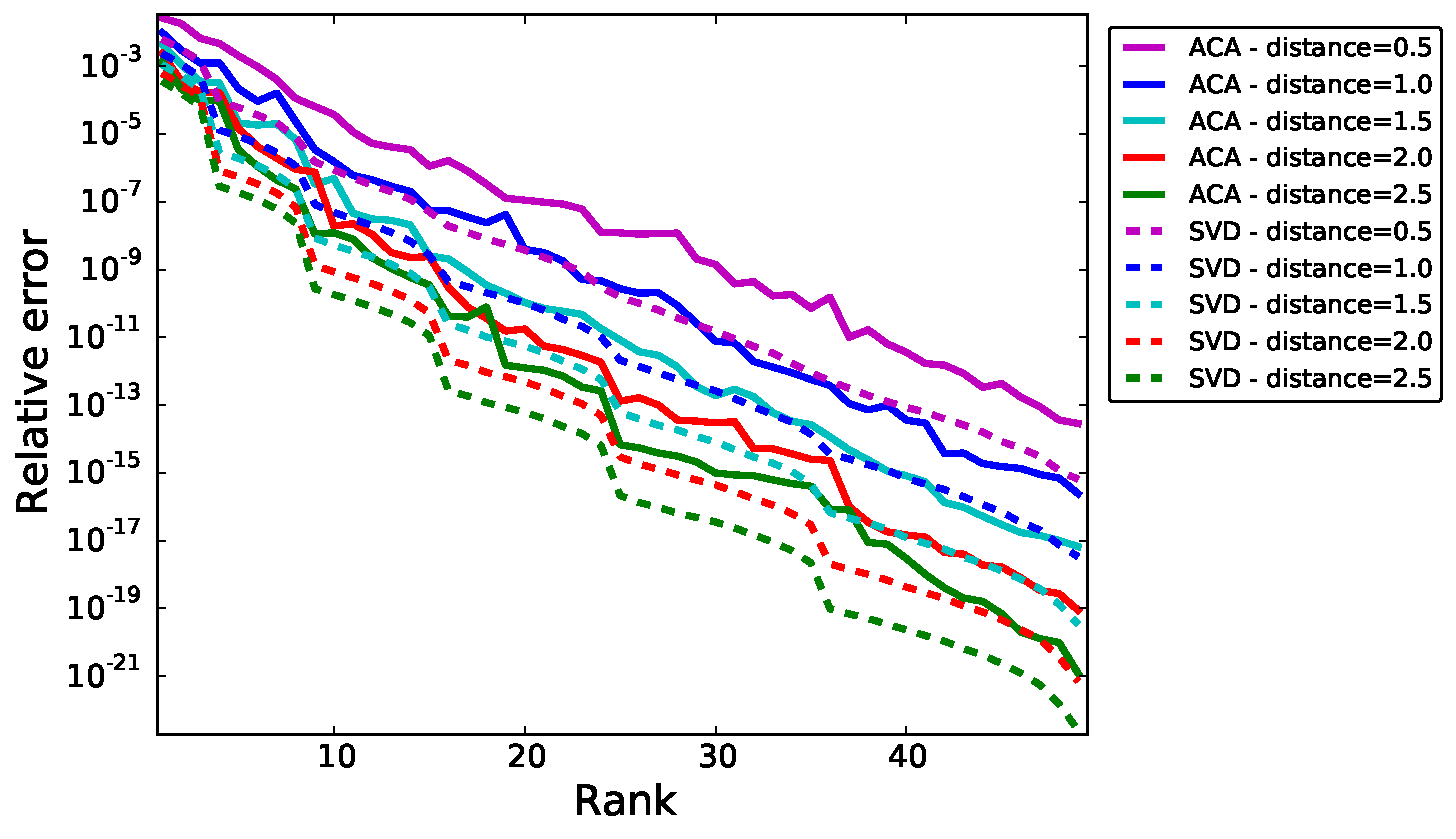
\includegraphics[width=.9\textwidth]{../images/graphe_output_err_decrease}
\caption{Relative error on the interaction matrix between two clusters of points with ACA (solid lines) and SVD (dashed lines) varying the distance between the two clusters.}
\label{fig:err_decrease}
\end{figure}




